\documentclass[a4paper, 12pt]{article}

\newcommand{\languages}{english, french}

%%%%% Tools

\usepackage{comment}
\usepackage{lipsum}
\usepackage{xstring}

%%%%% Document

\usepackage[pdfusetitle]{hyperref}

\usepackage{geometry}
\geometry{paper=a4paper,top=2.5cm,bottom=2.5cm,right=2.5cm,left=2.5cm}

\usepackage{fancyhdr}
%\pagestyle{fancy}
%\fancyhead[L]{}
%\fancyhead[R]{\leftmark}
%\fancyfoot[C]{\thepage}
%\renewcommand{\headrulewidth}{0pt}

%%%%% Text

\usepackage[utf8]{inputenc}
\usepackage[T1]{fontenc}
\edef\restoreparindent{\parindent=\the\parindent\relax}
\usepackage[parfill]{parskip}
%\restoreparindent
\usepackage{csquotes}

\newlength{\mytextsize}
\makeatletter
\setlength{\mytextsize}{\f@size pt}
\makeatother

%%%%% Languages

\ifx\languages\undefined
	\usepackage[english]{babel}
\else
	\usepackage[\languages]{babel}
\fi

% english

\addto\captionsenglish{\def\figurename{Figure}}
\addto\captionsenglish{\def\tablename{Table}}

\def\st{\text{s.t.}}

% french

\frenchbsetup{StandardLists=true}

\addto\captionsfrench{\def\figurename{Figure}}
\addto\captionsfrench{\def\tablename{Table}}
\addto\captionsfrench{\def\proofname{Preuve}}

\def\tq{\text{t.q.}}
\def\cad{c.-à-d.}
\def\Cad{C.-à-d.}

%%%%% Styles

\usepackage[skip=\mytextsize]{caption}
\usepackage{float}
\usepackage{mdframed}
\usepackage{enumitem}
\usepackage{eurosym}
\usepackage{color}

\newcommand\caaption[1]{\caption{#1}\vspace{-1\mytextsize}}

%%%%% Mathematics

\usepackage{amsmath}
\usepackage{amssymb}
\usepackage{amsfonts}
\usepackage{bm}
\usepackage{esint}
\usepackage[makeroom]{cancel}

\newcommand{\fact}[1]{#1!}
\newcommand{\e}[1]{\mathbf{e}_{#1}}
\newcommand{\deriv}{\mathrm{d}}
\DeclareMathOperator{\tr}{tr}


%%%%% SI units

\usepackage[squaren,Gray,cdot]{SIunits}
\usepackage{sistyle}

\IfStrEq{\languagename}{french}{
	\SIdecimalsign{,}
}

%%%%% Chemistry

\usepackage[version=4]{mhchem}

%%%%% Table & Figure

\usepackage{subcaption}

\usepackage{array}
\usepackage{tabularx}
\usepackage{multirow}
\usepackage{multicol}
\newcolumntype{M}[1]{>{\centering\arraybackslash}m{#1}}
%\setlength\extrarowheight{0em}
\renewcommand{\arraystretch}{1.3}

\usepackage{pgfplots}
\usepackage{tikz}
\usetikzlibrary{shapes.geometric, positioning}
\usepackage{graphics}
\usepackage{graphicx}
\pgfplotsset{axis on top, compat = 1.3}

%%%%%% Theorems and Definitions

\usepackage{amsthm}
\usepackage{thmtools}

\def\lgthm{Theorem}
\def\lglem{Lemma}
\def\lgprop{Proposition}
\def\lgdefn{Definition}
\def\lghyp{Hypothesis}
\def\lgquest{Question}
\def\lgansw{Answer}
\def\lgexpl{Example}
\def\lgrmk{Remark}
\def\lgnote{Note}
\def\lgtip{Tip}

\IfStrEq{\languagename}{french}{
	\def\lgthm{Théorème}
	\def\lglem{Lemme}
	\def\lgprop{Proposition}
	\def\lgdefn{Définition}
	\def\lghyp{Hypothèse}
	\def\lgquest{Question}
	\def\lgansw{Réponse}
	\def\lgexpl{Exemple}
	\def\lgrmk{Remarque}
	\def\lgnote{Note}
	\def\lgtip{Conseil}
}

\theoremstyle{plain}
\newtheorem{thm}{\lgthm}[section]
\newtheorem{lem}{\lglem}[section]
\newtheorem{prop}{\lgprop}[section]

\theoremstyle{definition}
\newtheorem{defn}{\lgdefn}[section]
\newtheorem{hyp}{\lghyp}[section]
\newtheorem{quest}{\lgquest}[]

\declaretheorem[
name=\lgansw,
qed={\lower-0.3ex\hbox{$\triangle$}},
within=quest
]{answ}

\declaretheorem[
name=\lgexpl,
qed={\lower-0.3ex\hbox{$\triangle$}},
within=section
]{expl}

\theoremstyle{remark}
\newtheorem*{rmk}{\lgrmk}
\newtheorem*{note}{\lgnote}
\newtheorem*{tip}{\lgtip}

\begingroup
\makeatletter
\@for\theoremstyle:=definition,remark,plain\do{%
	\expandafter\g@addto@macro\csname th@\theoremstyle\endcsname{%
		\addtolength\thm@preskip\parskip
	}%
}
\endgroup

%%%% Others

\renewcommand{\qedsymbol}{$\blacksquare$}

\newcommand{\mytableofcontents}{
	\newpage
	\pagenumbering{roman}
	\tableofcontents
	\newpage
	\pagenumbering{arabic}
}

%%%%%%%%%%%%%%%%%%%

%%%%%%%%%%%%%%%%%%%

\newcommand{\imgheader}{resources/pdf/logo-uliege.pdf}
\newcommand{\institution}{University of Liege}

\title{Pacman - Search agent}
\newcommand{\subtitle}{Introduction to artificial intelligence}

\author{Maxime \textsc{Meurisse} (20161278)\\Valentin \textsc{Vermeylen} (20162864)\\}

\newcommand{\context}{3rd year of Bachelor Civil Engineer}
\date{Academic year 2018-2019}

%%%%%%%%%%%%%%%%%%%

\begin{document}
    \newgeometry{margin = 2.5cm}
\makeatletter
\begin{titlepage}
	\begin{minipage}[t][0.425\textheight][t]{\textwidth}
		\begin{center}
			\includegraphics[height=0.15\textheight]{\imgheader}
			\vfill
			{\huge \textsc{\institution}}
			\vfill
		\end{center}
	\end{minipage}
	\vfill
	\begin{minipage}{\textwidth}
		\hspace{6pt}
		\begin{mdframed}[linewidth = 2pt, innertopmargin = 12pt, innerbottommargin = 12pt, leftline = false, rightline = false]
			\begin{center}
				{\huge \bfseries \@title}
			\end{center}
		\end{mdframed}
		\hspace{6pt}
	\end{minipage}
	\vfill
	\begin{minipage}[b][0.425\textheight][t]{\textwidth}
		\begin{center}
			{\LARGE \subtitle}
			\vfill
			{\large \@author\space}
			\vfill
			{\large \context \\[6pt] \@date}
		\end{center}
	\end{minipage}
\end{titlepage}
\makeatother
\restoregeometry
	
	%% Section 1: formalization of the problem %%
	\section{Formalization of the problem}
	
	\subsection{Formalization as a search problem}
	First, we define the agent. In this problem, the Pacman player will be a search agent, implemented as a \texttt{PacmanAgent} class.\par
	
	Second, we define the state of the agent. This state consists of a series of information, including Pacman's position in the labyrinth and the boolean state of all food dots.\par
	
	A search problem consists of an initial state of the agent, a description of the possible actions for an agent state, a transition model that returns the new state of the agent after execution of an action, a goal test and a path cost.\par
	
	Let us specify these components in the case of our problem:
	\begin{itemize}
	    \item initial state of the agent: the starting position of Pacman in the grid (defined by the layout, i.e. the game grid with food dots) and a boolean matrix of food dots;
	    \item possible actions for a given state: Pacman can move in 4 directions: North, South, West and East or may not move. If a move leads Pacman into a wall, it is said to be an illegal move, otherwise it is a legal move;
	    \item transition model: thanks to one of the four previous actions, Pacman updates its position in the labyrinth and possibly updates the boolean state of a food dot. The new state of Pacman is a successor of his previous state if Pacman does a legal move;
	    \item goal test: check if all the food dots have been eaten, i.e. if all the food dots matrix is composed of false boolean value.
	    \item path cost: each single movement has the same cost but a sequence of movements can lead to different scores. The path cost is defined by Pacman's score.
	\end{itemize}
	
	
	%% Section 2: performance of algorithms %%
	\section{Performance of algorithms}
	The algorithms were run\footnote{The algorithms were run on a machine equipped with an 3.1 GHz Intel Core i7 processor with 16 GB of RAM.} on the different layouts to study and compare their performance. All reported data is an average of 10 similar data.
	
	\newpage
	
	\begin{figure}[!ht]
    	\centering
        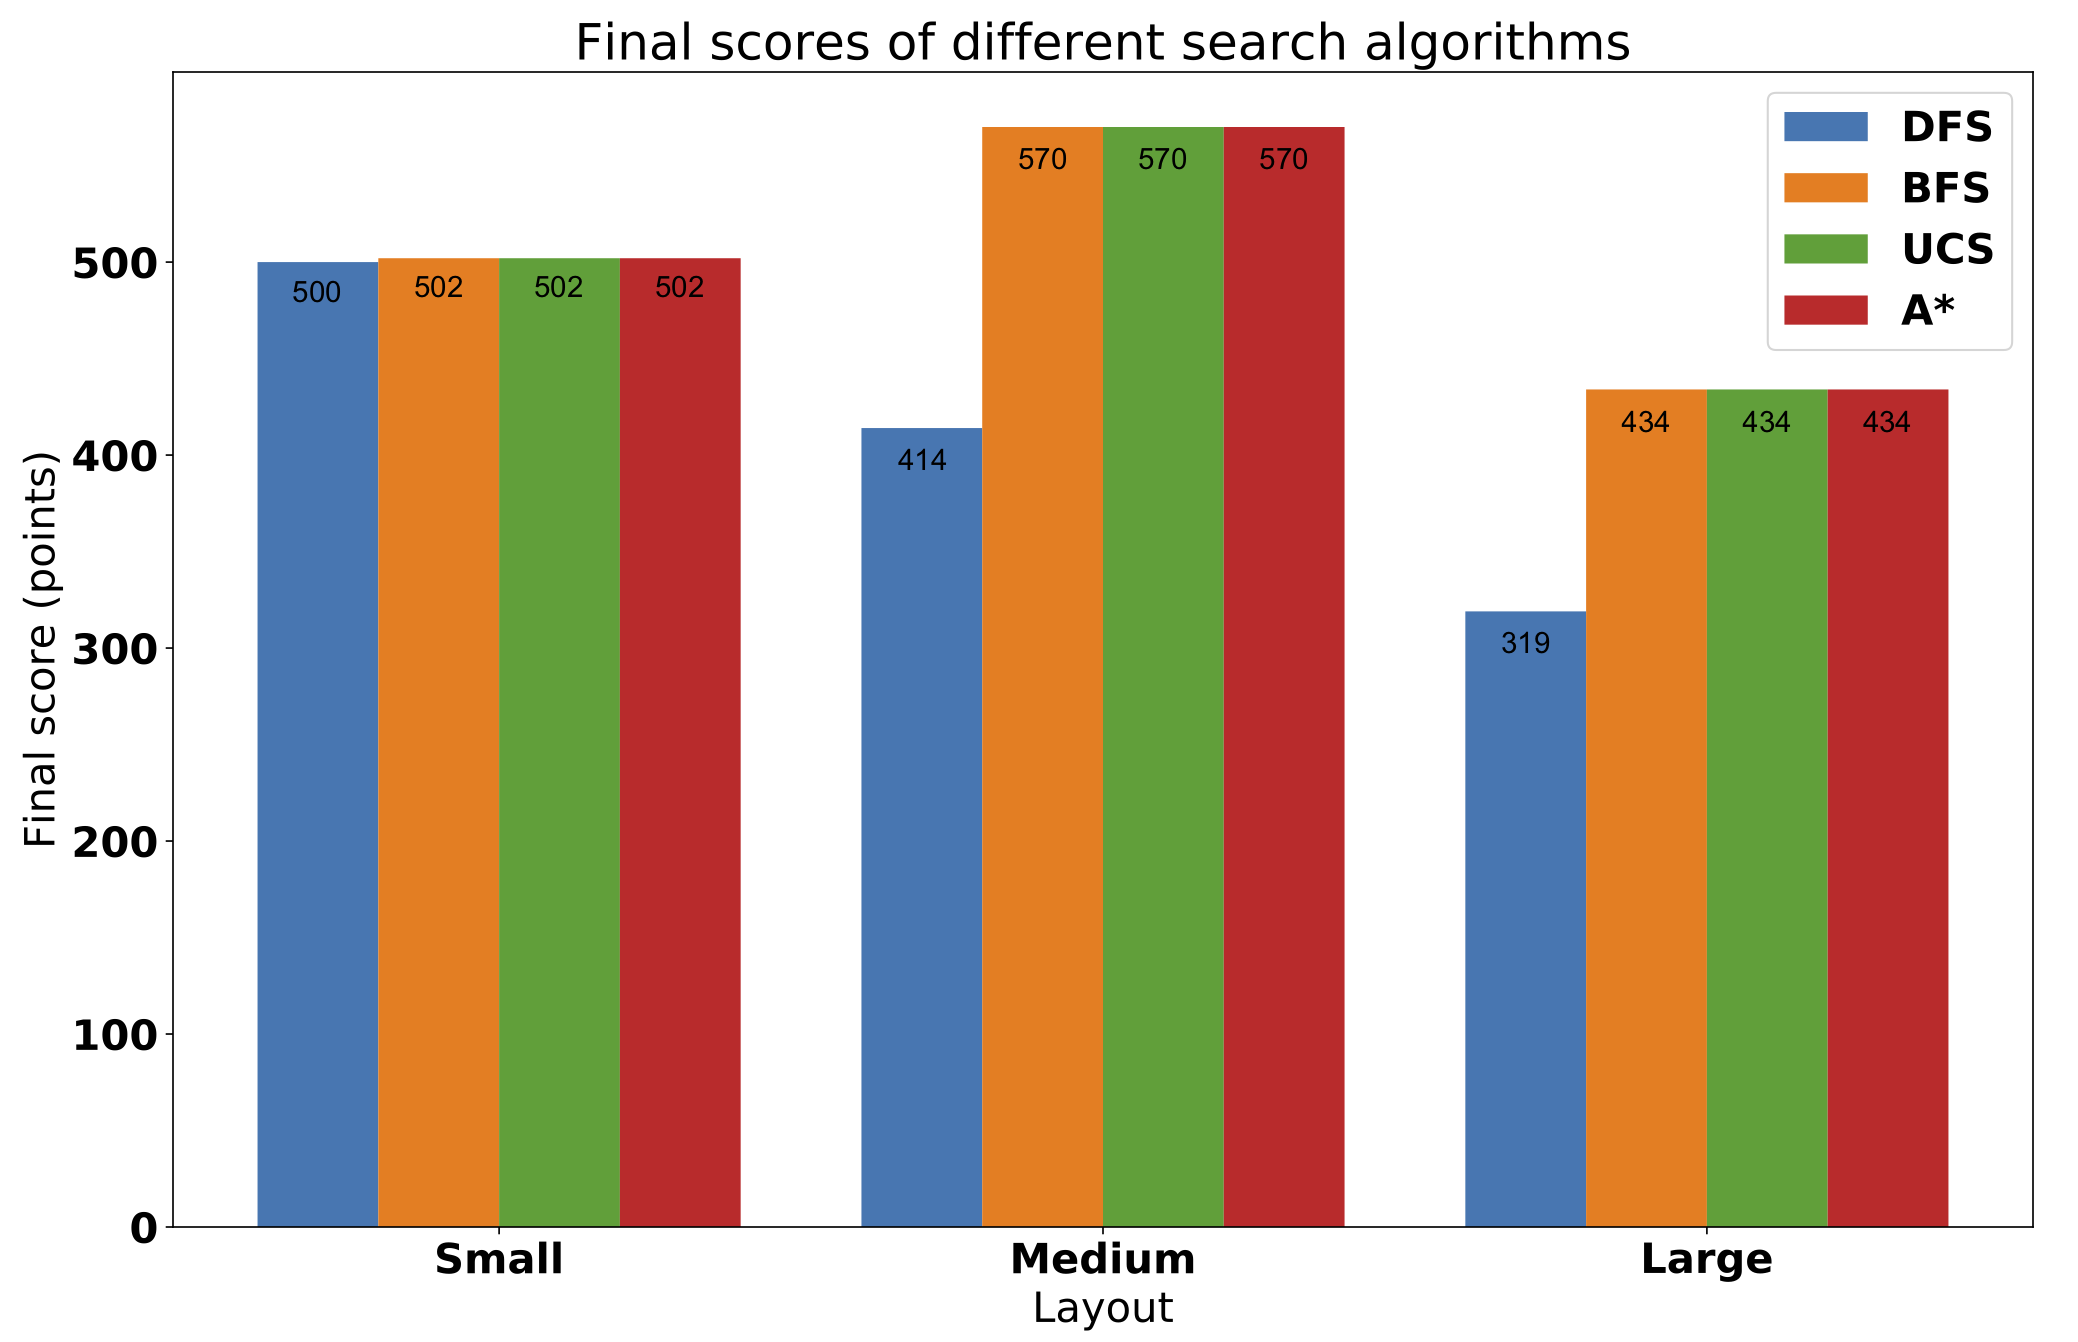
\includegraphics[width=0.9\textwidth]{resources/png/scores.png}
        \caption{Comparison of the final scores of the algorithms on the different layouts.}
        \label{fig:scores}
    \end{figure}
    
    \begin{figure}[!ht]
    	\centering
        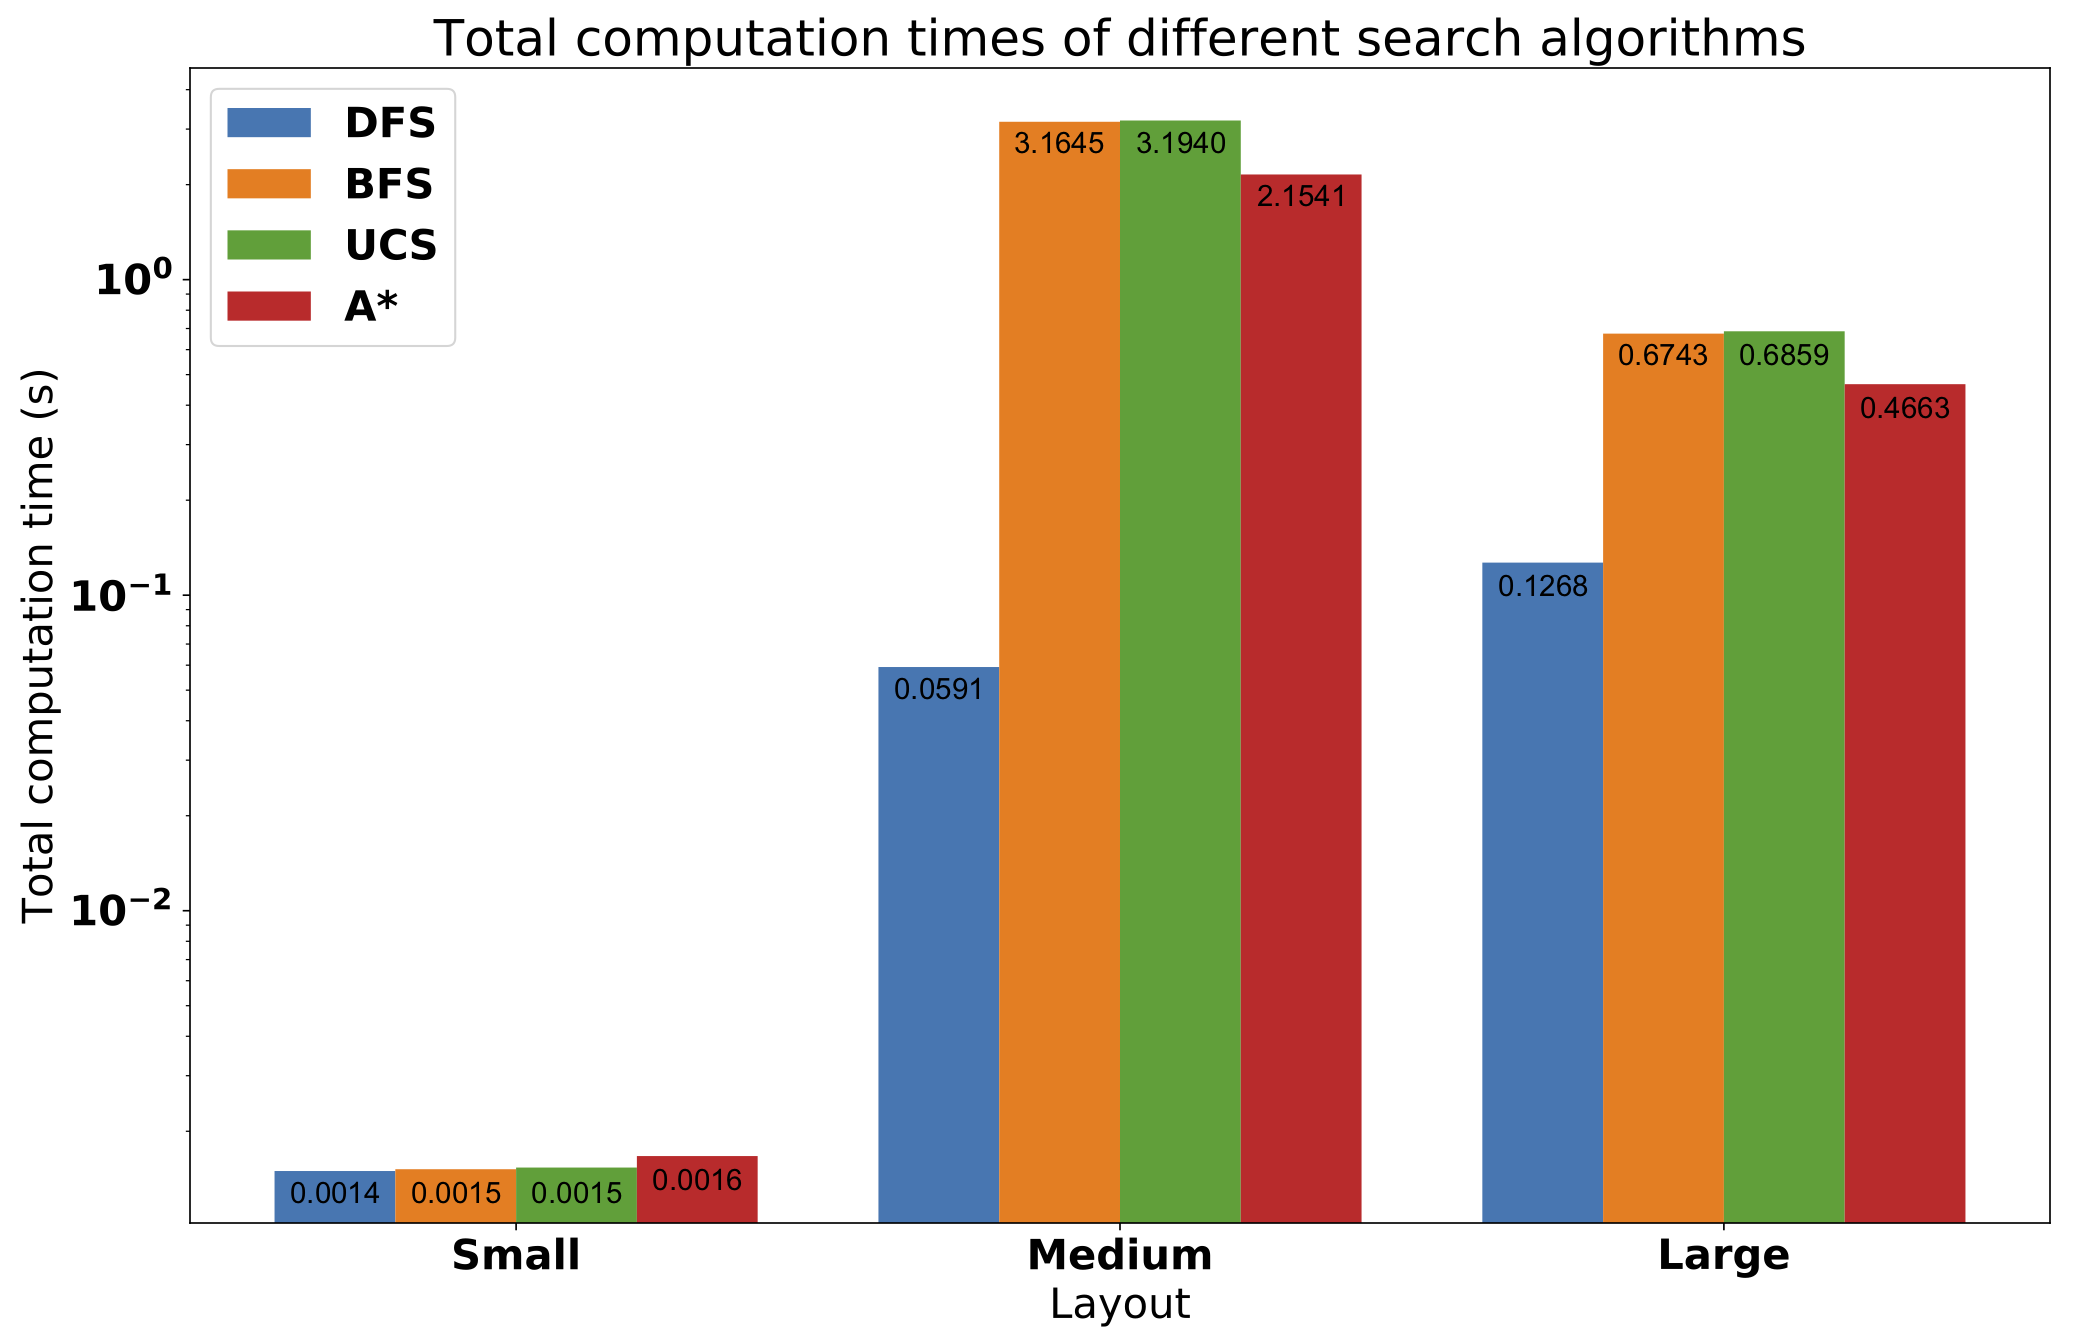
\includegraphics[width=0.9\textwidth]{resources/png/times.png}
        \caption{Comparison of the total computation time of the algorithms on the different layouts.}
        \label{fig:times}
    \end{figure}
	
	\begin{figure}[!ht]
    	\centering
        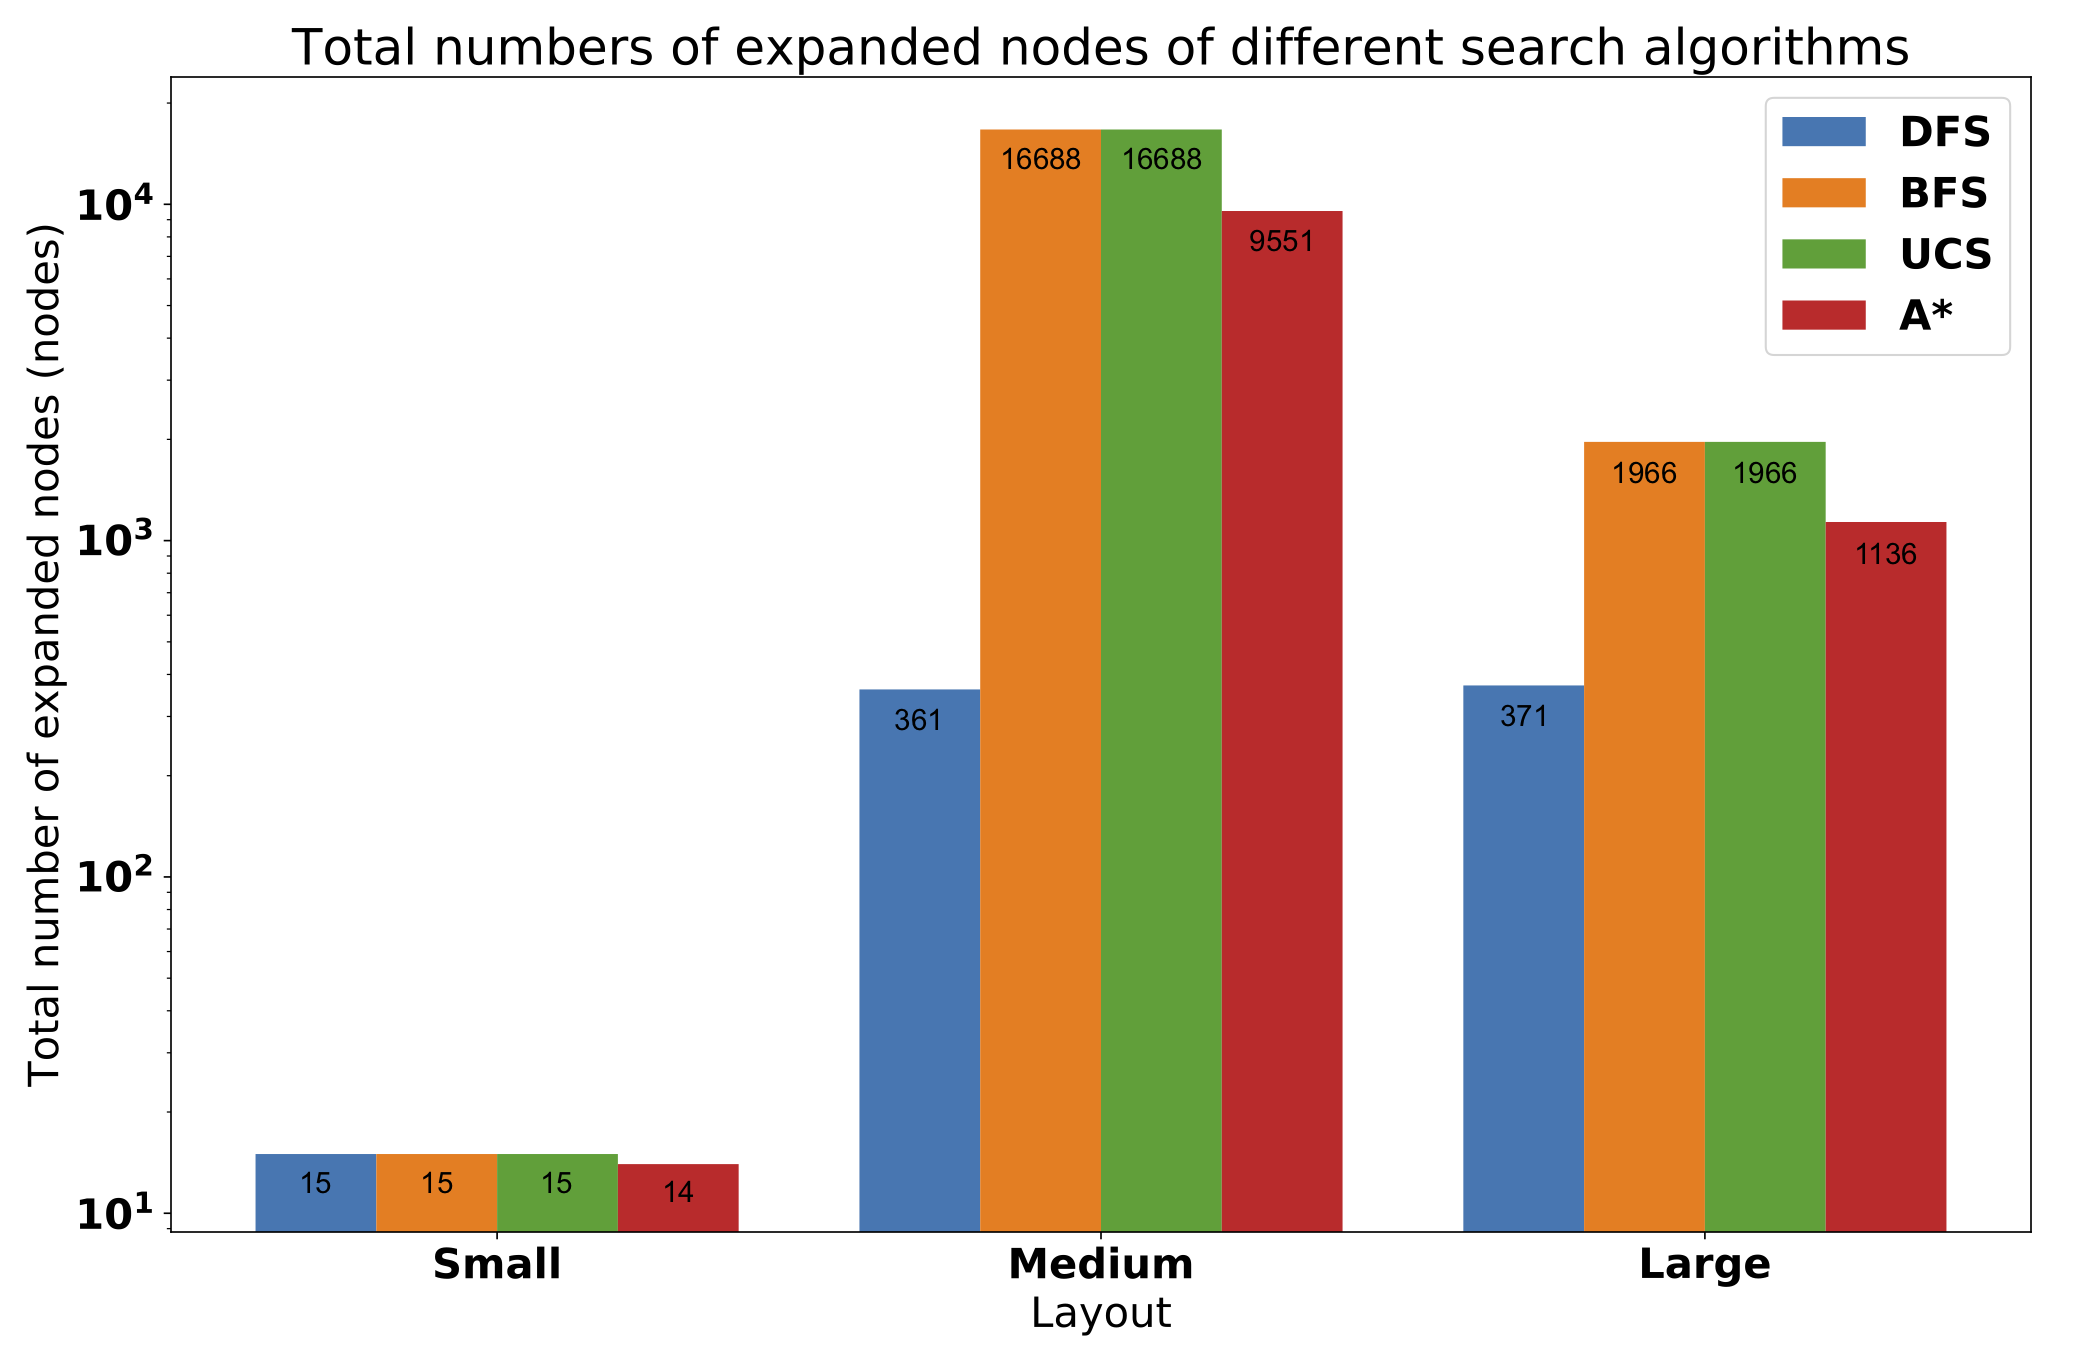
\includegraphics[width=0.9\textwidth]{resources/png/nodes.png}
        \caption{Comparison of the total number of expanded nodes of the algorithms on the different layouts.}
        \label{fig:nodes}
    \end{figure}
	
	
	%% Section 3: discussion %%
	\section{Discussion}
	As a general observation for all agents, the medium layout requires the most computation time, and that is due to the fact that there are a lot of food dots to eat, so the solutions are less direct, and Pacman needs to explore almost all cells, and sometimes more than once.\par
	
	The large layout, on the other hand, only have 4 dots. So, while it has larger dimensions than the medium one, the computation time is smaller because the path to the solution is more direct (less convoluted).
	
	\subsection{Depth-first search}
	As can be seen in figure \ref{fig:scores}, \texttt{DFS} is not optimal in any of the layout on which it has been tested. We can easily understand why : \texttt{DFS} goes as deep as it can in the state tree and, therefore, finds the leftmost deepest solution, regardless of its optimality. And, as each branch corresponds to an action taken in the maze, a deep solution corresponds to a long sequence of actions. Thus, the score decreasing with the number of actions of the sequence, a deep solution means a non-optimal score.\par
	
	However, as it concentrates its search on the left part of the tree, it finds a solution quite quickly, thanks to the fact that an infinite number of solutions exist in this project (so we can be assured that \texttt{DFS} will find one in the left part of the search tree). That provides us with an algorithm that is significantly faster, computationally-wise, than all the other ones, but that provides a worst solution, and these two aspects are amplified as the layout gets larger.\par
	
	The number of expanded nodes being directly related to the computation time, the analysis conducted just above holds for that aspect too, and is not mentioned for the other agents.
	
	\subsection{Breadth-first search and Uniform cost search}
	As the results show, \texttt{UCS} and \texttt{BFS} provide an optimal solution (best possible score) but with a large number of expanded nodes, and more slowly than the other algorithms, and this for all layouts.\par
	
	They have the same results everywhere, and this comes from the way we implemented the priority. Indeed, we used the length of the list of actions leading to a state as priority, which means that \texttt{UCS} behaves exactly as \texttt{BFS}, exploring the shallowest nodes first.\par
	
	We initially used the opposite of the cost of a state as priority, but we realized that it was not optimal. The score could change its sign and so the priority did not truly reflect the best path possible (the fact that eating a dot only gave 10 point and finishing the game gave several hundreds accounted for that too). However, the number of nodes expanded and the computation time were decreased.
	
	\subsection{A* (and his associated heuristic)}
	We chose as heuristic for \texttt{A*} the sum of the length of the sequence of actions leading to a state and the Manhattan distance to the farthest food dot. As we have seen in the theoretical course, the Manhattan distance is an admissible heuristics. That means that the score obtained via \texttt{A*} is optimal, and thus are the ones obtained via \texttt{UCS} (and \texttt{BFS} consequently), as can be seen on the graphs.\par
	
	Regarding the computation time (and the number of nodes expanded), \texttt{A*} is better than \texttt{BFS} and \texttt{UCS}, but not as effective as \texttt{DFS}, and this for all layouts.\par
	
	We can see that it is the algorithm that takes the less computation time amongst those that provide the best score.\par
	
	An observation we made is that, if we take the Manhattan distance to the nearest node instead of the farthest, the computation time and number of expanded nodes is multiplied by 6 on the medium layout, but the score is still optimal. That can be explained by the fact that a lot of states will then have the same priority, as the distance to the nearest food is much more likely to be equal to that of another state than in the case of the farthest dot. The search agent will be less well-guided (the contour of the search will look more like a circle than an elongated ellipse), and so have poorer performance. However, as the heuristic is still admissible, the score will be optimal.
	
	\subsection{Conclusion}
	Based on the previous discussions, we can conclude that the algorithm \texttt{A*}, in general, provides the optimal solution (in terms of score, nodes expanded and total computation time).\par
	
	The \texttt{DFS} algorithm is the fastest and provides an almost optimal solution for small layouts (in any case with a small number of food dots to eat). It could be used in these cases, because the solution would be acceptable and the computation time reduced, but would quickly become bad for other layouts.\par
	
	The \texttt{UCS} and \texttt{BFS} algorithms provide, in our case, an optimal score, but with a long computation time and many expanded nodes. So, their use is limited: they quickly become unusable on very large layout. We will therefore prefer the algorithm \texttt{A*}.
\end{document}
